\documentclass[11pt]{beamer}
\usepackage{etex}
\usetheme[
%%% options passed to the outer theme
%    progressstyle=fixedCircCnt,   %either fixedCircCnt, movCircCnt, or corner
%    rotationcw,          % change the rotation direction from counter-clockwise to clockwise
%    shownavsym          % show the navigation symbols
  ]{AAUsimple}

% If you want to change the colors of the various elements in the theme, edit and uncomment the following lines
% Change the bar and sidebar colors:
%\setbeamercolor{AAUsimple}{fg=green!20,bg=green}
%\setbeamercolor{sidebar}{bg=red!20}
% Change the color of the structural elements:
%\setbeamercolor{structure}{fg=red}
% Change the frame title text color:
%\setbeamercolor{frametitle}{fg=blue}
% Change the normal text color background:
%\setbeamercolor{normal text}{fg=black,bg=gray!10}
% ... and you can of course change a lot more - see the beamer user manual.

\usepackage[utf8]{inputenc}
\usepackage[english]{babel}
\usepackage[T1]{fontenc}
% Or whatever. Note that the encoding and the font should match. If T1
% does not look nice, try deleting the line with the fontenc.
\usepackage{helvet}
\usepackage{xcolor}

%use for graphics
\usepackage{calc}
\usepackage{ifthen}
\usepackage{amsmath,amsfonts,amssymb,amsthm}
\usepackage{mathtools}

\usepackage{tikz}
\usetikzlibrary{arrows, automata, positioning}
\DeclarePairedDelimiter{\ceil}{\lceil}{\rceil}
\DeclarePairedDelimiter{\floor}{\lfloor}{\rfloor}
\DeclarePairedDelimiter{\tuple}{\langle}{\rangle}
\newcommand{\darrow}{\, \downarrow \!\!}
\newcommand{\uarrow}{\, \uparrow \!\!}

%other package for graphics

%\usepackage{pstricks}
%\usepackage{pstricks-add}

%\usepackage{pst-plot}
\usepackage{xcolor,colortbl}

\newcommand{\mc}[2]{\multicolumn{#1}{c}{#2}}
\definecolor{Gray}{gray}{0.85}

\newcolumntype{a}{>{\columncolor{Gray}}c}
\newcolumntype{b}{>{\columncolor{white}}c}

% command for slices graphic
\newcommand{\slice}[4]{
  \pgfmathparse{0.5*#1+0.5*#2}
  \let\midangle\pgfmathresult

  % slice
  \draw[thick,fill=black!10] (0,0) -- (#1:1) arc (#1:#2:1) -- cycle;

  % outer label
  \node[label=\midangle:#4] at (\midangle:1) {};

  % inner label
  \pgfmathparse{min((#2-#1-10)/110*(-0.3),0)}
  \let\temp\pgfmathresult
  \pgfmathparse{max(\temp,-0.5) + 0.8}
  \let\innerpos\pgfmathresult
  \node at (\midangle:\innerpos) {#3};
}
% colored hyperlinks
\newcommand{\chref}[2]{%
  \href{#1}{{\usebeamercolor[bg]{AAUsimple}#2}}%
}


\title{Data structures for Partially Ordered Sets}  % could also be a conference name
\subtitle{Prepatory work for the master thesis}

\date{June 7, 2018}

\author{
  Hakim Boulahya
}

% - Give the names in the same order as they appear in the paper.
% - Use the \inst{?} command only if the authors have different
%   affiliation. See the beamer manual for an example

\institute[
%  {\includegraphics[scale=0.2]{aau_segl}}\\ %insert a company, department or university logo
  Faculty of Science
  Université Libre de Bruxelles
  Belgium
] % optional - is placed in the bottom of the sidebar on every slide
{% is placed on the bottom of the title page
  Département d'Informatique \\
  Université Libre de Bruxelles \\
  Belgium

  %there must be an empty line above this line - otherwise some unwanted space is added between the university and the country (I do not know why;( )
}

% specify a logo on the titlepage (you can specify additional logos an include them in
% institute command below
\pgfdeclareimage[height=1.5cm]{titlepagelogo}{../images/logoULB} % placed on the title page
\titlegraphic{% is placed on the bottom of the title page
  \pgfuseimage{titlepagelogo}
%  \hspace{1cm}\pgfuseimage{titlepagelogo2}
}
\definecolor{firstcolor}{RGB}{0, 76, 146}
\definecolor{secondcolor}{RGB}{43,46,62}
\definecolor{thirdcolor}{RGB}{180,200,212}

\begin{document}
% the titlepage
{\aauwavesbg%
\begin{frame}[plain,noframenumbering] % the plain option removes the header from the title page
  \titlepage
\end{frame}}
%%%%%%%%%%%%%%%%
%%%%%%%%%%%%%%%%

% TOC
\begin{frame}{Contents}{}

%\centering \textit{\large The involvment of Facebook in the learning process}
\begin{block}{}
  \begin{enumerate}
    \item \textcolor{firstcolor}{\textbf{Introduction}}
     Subject and motivations
    \item \textcolor{firstcolor}{\textbf{Definitions}}
     Poset and antichains
     \item \textcolor{firstcolor}{\textbf{Existing implementation}}
    \item \textcolor{firstcolor}{\textbf{Objective}}
     Requirements and overview
  \end{enumerate}
\end{block}

\end{frame}

%%%%%%%%%%%%%%%% HAKIM %%%%%%%%%%%%%%%%%%%%%%%%%%%%
\section{Motivation}
\begin{frame}{Introduction}{}
    \begin{block}{Subject}
        \begin{itemize}
            \item Implement data structures to represent partially ordered sets
            \item Main focus on antichain-based algorithms in automata theory
        \end{itemize}
    \end{block}
    \begin{block}{Motivations}
        \begin{itemize}
            \item There exists new algorithms that uses antichains:
            \begin{itemize}
                \item Model checking
                \item Synthesis problem
                \item Language universality
            \end{itemize}
            \item There is a need for an efficient implementation of antichains
        \end{itemize}
    \end{block}
    % \begin{block}{Facebook as a learning tool}
    %   \pause
    %   \begin{itemize}
    %     \item A new way to learn/teach ?
    %     \item Improving learning ?
    %   \end{itemize}
    % \end{block}
    % \pause
    % \begin{block}{Survey}
    %   \pause
    %   \begin{itemize}
    %     \item Students habits \& expectations
    %     \item Efficient use of \textcolor{secondcolor}{Facebook}
    %   \end{itemize}
    % \end{block}
    % \pause
    % \begin{block}{\center \textbf{GOAL}}
    %  \center \large \textcolor{black}{Explore the potential benefits of Facebook for the learning process}
    %  \end{block}
\end{frame}

\section{Definitions}

\begin{frame}{Data Structures}{Definitions}
    \begin{block}{Partial order}
        A partial order $\preceq$ on a set $S$ is a binary relation
        $\preceq \subseteq S \times S$
        that is reflexive, transitive and antisymmetric.
    \end{block}
    \begin{block}{Partially ordered set (or poset)}
    A partially ordered set is a pair $\tuple{S, \preceq}$
    where $S$ is a set, and $\preceq$ a partial order on $S$.
    \end{block}
    \begin{block}{Antichains}
    An antichain $\alpha$ is a set of incomparable
    elements of poset $\tuple{S, \preceq}$ w.r.t. to $\preceq$.
    \end{block}

\end{frame}

\begin{frame}{Data Structures}{Operations}
    \begin{block}{Interestring operations}
    \begin{itemize}
        \item \textbf{Lower closure} of an antichain $\alpha$
        on $S$, denoted $\darrow{\alpha}$,
        is the set of all elements of $S$ that are smaller or equal
        to an element of $\alpha$
        \item \textbf{Appartenance} $s \in \darrow \alpha_1$
        \item \textbf{Inclusion} $\darrow \alpha_1 \subseteq \darrow \alpha_2$
        \item \textbf{Union} $ \darrow \alpha_1 \ \cup \darrow \alpha_2 =
        \darrow \ceil{\alpha_1 \cup \alpha_2}$
        \item \textbf{Intersection} $\darrow \alpha_1 \ \cap \darrow \alpha_2$
    \end{itemize}
    \end{block}

\end{frame}

\begin{frame}{Data Structures}{Example}

    \begin{columns}[T]
     \begin{column}{.4\textwidth}
         \begin{block}{Example}
         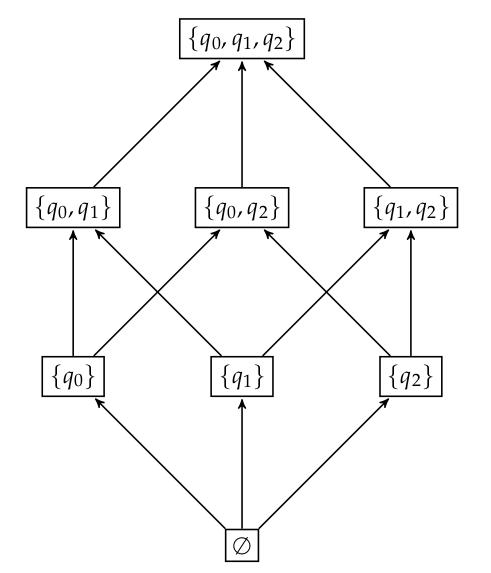
\includegraphics[scale=0.3]{../images/example}
         \end{block}
       \end{column}
       \begin{column}{.6\textwidth}
           \begin{block}{}
               \begin{itemize}
                   \item Poset is $\tuple{2^Q, \subseteq}$, where
                   $Q = \{q_0, q_1, q_2\}$
                   \item $\alpha = \{\{q_0, q_2\}, \{q_1, q_2\}\}$ is an
                   antichain
                   \item Can retrieve all subset of cardinality 1 using
                   the closure on the antichain: $\darrow{\alpha}$
                   \item $\darrow{\alpha} = \{\{q_0\}, \{q_1\}, \{q_2\},
                   \{q_0, q_2\}, \{q_1, q_2\}\}$
               \end{itemize}
           \end{block}
       \end{column}
   \end{columns}

\end{frame}

\section{Existing implementation}

\begin{frame}{Existing implementations}
    \begin{block}{Do implementation already exists ?}
        Yes, 2 for antichains:
        \begin{enumerate}
            \item \textbf{AaPAL}: Antichains implementation in $C$
            \begin{itemize}
                \item More of an API: user must implement
                comparison and intersection
            \end{itemize}
            \item Antichains for the Dedekind number problem
            \begin{itemize}
                \item Bitarray represention (a bit is a subset)
                \item Can only be applied to natural numbers
            \end{itemize}

        \end{enumerate}
    \end{block}
\end{frame}

\section{Objective}

\begin{frame}{Objective}{Requirements}
    \begin{block}{Requirements}
        \begin{itemize}
            \item \texttt{Owl} library: an automata library
            \item But symbolic antichain-based algorithm are missing
            (including antichain data structures)
            \item Implementation in \texttt{Java 10}
        \end{itemize}

    \end{block}
\end{frame}

\begin{frame}{Objective}{}
    \begin{block}{What to do ?}
        \begin{itemize}
            \item Provide an API and implement it against \texttt{Owl}
            \item Provide some implementation for antichains depending
            on the universe of the sets
            \item Define the algorithms to test our antichains
            implementation against
            \item Study the performance of those implementations
        \end{itemize}

    \end{block}
\end{frame}


{\aauwavesbg
\begin{frame}[plain,noframenumbering]
  \finalpage{Thank you!}
\end{frame}}
%%%%%%%%%%%%%%%%

\end{document}
